\section{Strutture dati per insiemi disgiunti}

Una \textbf{struttura dati per insiemi disgiunti} mantiene una collezione:

$$C=\{S_1,S_2,...,S_k\}$$ 

di insiemi dinamici disgiunti. Ciascun insieme è identificato da un \textbf{rappresentante}, che è uno degli elementi dell'insieme. Ogni elemento di un insieme è rappresentato da un oggetto. Indicando con $x$ un oggetto, vogliamo supportare le seguenti operazioni:

\begin{itemize}

\item \textbf{MakeSet}: aggiunge alla struttura dati un nuovo insieme contenente solo l'elemento $x$. Si richiede che $x$ non compaia in nessun altro insieme della struttura;
\item \textbf{FindSet}: ritorna il rappresentante dell'insieme che contiene $x$;
\item \textbf{Union}: riunisce i due insiemi contenenti $x$ ed $y$ in un unico insieme.

\end{itemize}

\subsection{Rappresentazione tramite liste concatenate}

Il modo più semplice per rappresentare una collezione di insiemi disgiunti è usare una lista circolare per ciascun insieme. 

\begin{figure}[htpd]
\centering
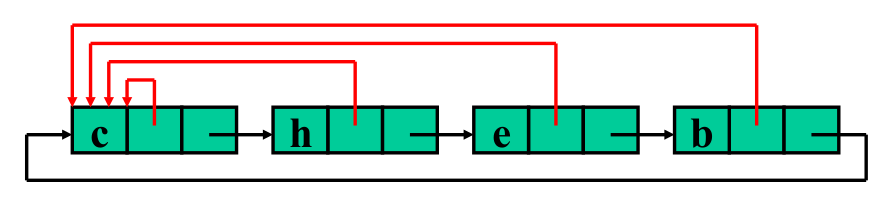
\includegraphics[width=100mm]{images/list-representation.png}
\caption{Rappresntazione con liste concatenate}
\end{figure}

I nodi hanno i seguenti campi:

\begin{itemize}

\item \textbf{info}: l'informazione contenuta nel nodo;
\item \textbf{r}: il puntatore al rappresentante;
\item \textbf{succ}: il puntatore al nodo successivo.

\end{itemize}

Le operazioni sono:

\begin{lstlisting}

MakeSet(x)
	x.r = x
	x.succ = x

\end{lstlisting}

\begin{figure}[htpd]
\centering
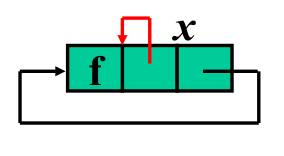
\includegraphics[width=50mm]{images/list-make-set.png}
\caption{Lista con l'operazione MakeSet}
\end{figure}

\begin{lstlisting}

FindSet(x)
	return x.r

\end{lstlisting}

\begin{figure}[htpd]
\centering
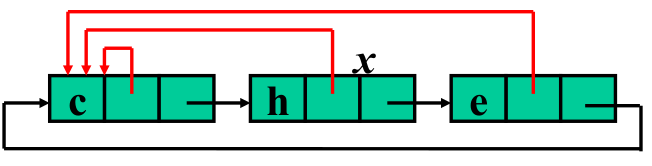
\includegraphics[width=50mm]{images/list-find-set.png}
\caption{Lista con l'operazione FindSet}
\end{figure}

\begin{lstlisting}[mathescape=true]

Union(x,y)
	// cambia i puntatori r nella lista di y
	y.r = x.r, z = y.succ
	while z $\neq$ y
		z.r = x.r, z = z.succ
	// concatena le due liste
	z = x.succ, x.succ = y.succ, y.succ = z

\end{lstlisting}

\begin{figure}[htpd]
\centering
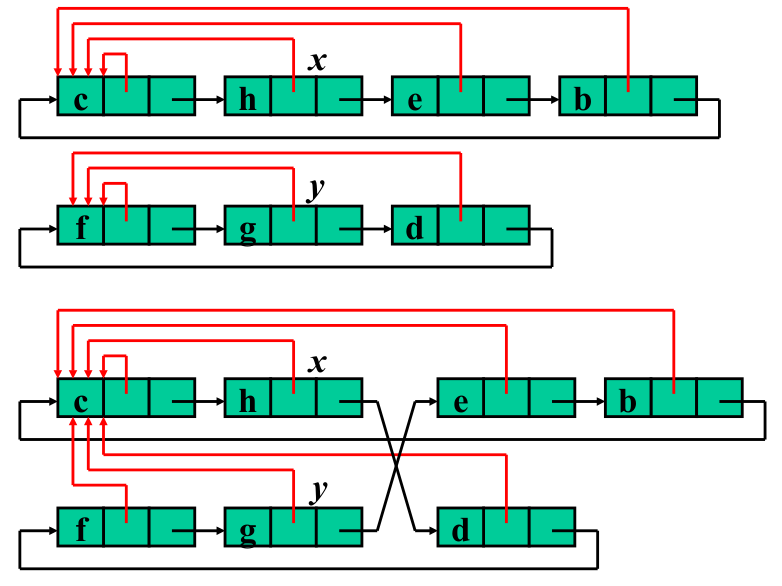
\includegraphics[width=50mm]{images/list-union.png}
\caption{Lista con l'operazione Union}
\end{figure}

La complessità di Union dipende dal numero di iterazioni richieste dal ciclo che cambia i puntatori al rappresentante dei nodi della lista contenente y. Quindi Union ha complessità uguale a: $O(n_2)$, dove $n_2$ è la lunghezza della seconda lista.

Consideriamo la sequenza di $2n-1$ operazioni su $n$ oggetti:
\linebreak
\linebreak

\begin{tabular}[htpd]{l c}
\centering

Operazione & Numero di oggetti aggiornati \\
\hline
MakeSet($x_1$) & 1 \\
MakeSet($x_2$) & 1 \\
... & ... \\
... & ... \\
MakeSet($x_n$) & 1 \\
Union($x_2,x_1$) & 1 \\
Union($x_3,x_2$) & 2 \\
Union($x_4,x_3$) & 3 \\
... & ... \\
... & ... \\
Union($x_n,x_{n-1}$) & $n-1$ \\

\end{tabular}

Il costo totale è proporzionale ad $n+n(n-1)/2$ ed è $\Theta(n^2)$ e le operazioni hanno costo ammortizzato $O(n)$.

\subsection{Euristica dell'unione pesata}

La complessità $\Theta(n^2)$ dell'esempio è dovuta al fatto che, in ogni Union, la seconda lista, quella che viene percorsa per aggiornare i puntatori al rappresentante, è la più lunga delle due.

L'euristica dell'\textbf{unione pesata} sceglie sempre la lista più corta per aggiornare i puntatori al rappresentante. Per poter fare ciò basta memorizzare la lunghezza della lista in un nuovo campo $L$ del rappresentante.

\begin{figure}[htpd]
\centering
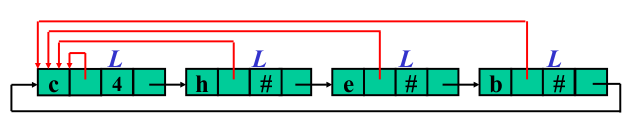
\includegraphics[width=100mm]{images/euristic1.png}
\end{figure}

Si può risparmiare memoria usando un campo booleano $b$ per distinguere il rappresentante.

\begin{figure}[htpd]
\centering
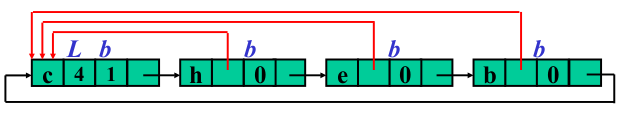
\includegraphics[width=100mm]{images/euristic2.png}
\end{figure}

Naturalmente occorre modificare le funzioni:

\begin{lstlisting}

MakeSet(x)
	x.b = true
	x.L = 1
	x.succ = x

\end{lstlisting}

\begin{lstlisting}

FindSet(x)
	if x.b
		return x
	else return x.r

\end{lstlisting}

\begin{lstlisting}[mathescape=true]

Union(x,y)
	x = FindSet(x)
	y = FindSet(y)
	// se la lista di x è piu' corta scambia x con y
	if x.L < y.L
		z = x, x = y, y = z
	x.L = x.L + y.L
	// cambia rappresentante alla lista di y
	y.b = false, y.r = x, z = y.succ
	while z $\neq$ y
		z.r = x, z = z.succ
	// concatena le due liste
	z = x.succ, x.succ = y.succ, y.succ = z

\end{lstlisting}

Con l'euristica dell'unione pesata una sequenza di $m$ operazioni delle quali $n$ sono MakeSet richiede tempo $O(m+n\log n)$. La complessità ammortizzata delle operazioni è quindi:

$$O(\frac{m+n\log n}{m})=O(1+\frac{n\log n}{m})=O(\log n)$$

Se il numero $n$ di MakeSet è molto minore di $m$ per cui $n\log n=O(m)$:

$$O(1+\frac{n\log n}{m}) = O(1)$$

\subsection{Rappresentazione con foreste}

Una rappresentazione più efficiente si ottiene usando \textbf{foreste di insiemi disgiunti}. Ogni insieme è rappresentato da un albero i cui nodi, oltre al campo info che contiene l'informazione, hanno soltanto un campo p che punta al padre.

\begin{figure}[htpd]
\centering
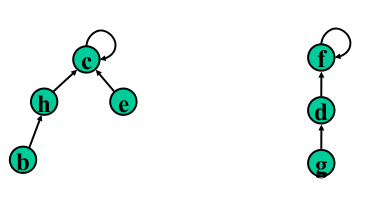
\includegraphics[width=50mm]{images/forest1.png}
\end{figure}

Implementazione semplice:

\begin{lstlisting}

MakeSet(x)
	x.p = x

\end{lstlisting}

\begin{lstlisting}[mathescape=true]

FindSet(x)
	while x.p $\neq$ x
		x = x.p
	return x

\end{lstlisting}

\begin{lstlisting}[mathescape=true]

Union(x,y)
	x = FindSet(x)
	y = FindSet(y)
	x.p = y

\end{lstlisting}

\begin{figure}[htpd]
\centering
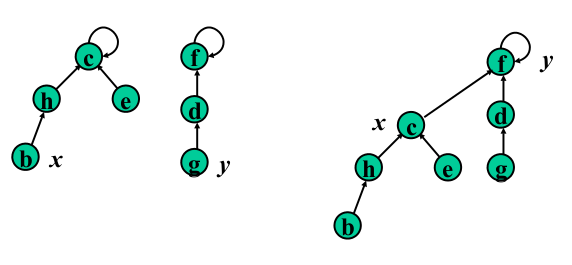
\includegraphics[width=50mm]{images/forest2.png}
\end{figure}

Sia nella rappresentazione con liste circolari che in quella con alberi non abbiamo indicato nessun puntatore esterno alla lista o all'albero. In realtà una struttura dati per insiemi disgiunti non è pensata per memorizzare dei dati ma soltanto per raggruppare in insiemi disgiunti dei dati che sono già memorizzati in qualche altra struttura: array, pila, lista, albero, tavola hash, ecc.

La complessità di FindSet(x) è pari alla lunghezza del cammino che congiunge il nodo $x$ alla radice dell'albero.

La complessità di Union è essenzialmente quella delle due chiamate FindSet(x) e FindSet(y).

Un esempio analogo a quello usato con le liste mostra che una sequenza di $n$ operazioni può richiedere tempo $O(n^2)$. 

Possiamo migliorare notevolmente l'efficienza usando due euristiche:
\linebreak
\linebreak
\textbf{L'euristica dell'unione per rango}: è simile a quella dell'unione pesate per le liste. In ogni nodo $x$ manteniamo un campo rank che è un limite superiore all'altezza del sottoalbero di radice $x$ ed è anche un'approssimazione del logaritmo del numero di nodi del sottoalbero. L'operazione Union mette la radice con rango minore come figlia di quella di rango maggiore.
\linebreak
\linebreak
\textbf{L'euristica della complessità dei cammini}: quando effettuiamo una FindSet(x) attraversiamo il cammino da $x$ alla radice. Posiamo approfittarne per far puntare alla radice dell'albero i puntatori al padre di tutti i nodi incontrati lungo il cammino. Le successive operazioni FindSet sui nodi di tale cammino risulteranno molto meno onerose.
\linebreak
\linebreak
L'implementazione con entrambe le euristiche è la seguente:

\begin{lstlisting}

MakeSet(x)
	x.p = x
	x.rank = 0

\end{lstlisting}

\begin{lstlisting}[mathescape=true]

FindSet(x)
	if x.p $\neq$ x
		x.p = FindSet(x.p)
	return x.p

\end{lstlisting}

\begin{figure}[htpd]
\centering
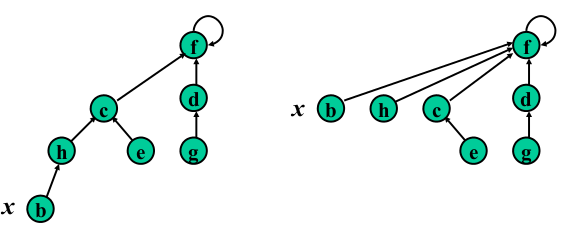
\includegraphics[width=50mm]{images/forest3.png}
\end{figure}

\begin{lstlisting}

Union(x,y)
	x = FindSet(x)
	y = FindSet(y)
	Link(x,y)

\end{lstlisting}

\begin{lstlisting}

Link(x,y)
	if x.rank > y.rank
		y.p = x
	else
		x.p == y
		if x.rank == y.rank
			y.rank = y.rank+1

\end{lstlisting}

\subsection{Proprietà dei ranghi}

Per ogni nodo $x$:

\begin{itemize}

\item $x$ viene creato come radice con $x.rank = 0$;
\item $x.rank$ aumenta soltanto finchè $x$ resta radice, dopo di che rimane invariato;
\item Se $x$ non è radice $x.rank<x.p.rank$;
\item $x.p.rank$ può solo aumentare;
\item Dopo aver eseguito $n$ operazioni $x.rank<n$.

\end{itemize}

\subsection{Le due funzioni $level(x)$ e $iter(x)$}

Per ogni nodo $x$ non radice definiamo due funzioni che ``misurano'' la differenza di rango tra $x$ e $x.p$:

$$level(x)=max\{k:x.p.rank \ge A_k(x.rank)\}$$
$$iter(x)=max\{i:x.p.rank \ge A_{level(x)}^{(i)}(x.rank)\}$$

Valgono le seguenti disuguaglianze:

$$ 0 \le level(x) < \alpha(n)$$
$$1\le iter(x) \le x.rank $$

\subsection{Calcolo del costo ammortizzato delle operazioni}

\subsubsection{MakeSet(x)}

$$\Delta\Phi_i=0$$
$$\hat{c}=c+\Delta\Phi_i=1=O(1)$$

\subsubsection{Link(x,y)}

Il potenziale $\Phi(x)$ dipende soltanto da $x.rank$ e $x.p.rank$. Quindi gli unici elementi il cui potenziale può cambiare sono $x$, $y$ e i figli di $y$. I figli di $y$ non sono radici e il loro potenziale non può aumentare. $x$ è radice e diventa figlio di $y$ ma il suo rango non cambia. Se $x.rank=0$:

$$\Delta\Phi_i(x)=\alpha(n)x.rank-\alpha(n)x.rank=0$$

Altrimenti:

$$\Delta\Phi_i(x)=(\alpha(n)-level(x))x.rank-iter(x)-\alpha(n)x.rank$$
$$-level(x)x.rank-iter(x)\le 0$$

$y$ rimane radice e $y.rank$ o rimane invariato o aumenta di 1. Quindi:

$$\Delta\Phi_i(y)=\alpha(n)y.rank_i-\alpha(n)y.rank_{i-1}\le \alpha(n)$$

Dunque $\Delta\Phi_i\le\alpha(n)$ ed il costo ammortizzato di Link è:

$$\hat{c}=c+\Delta\Phi_i\le 1 +\alpha(n)=O(\alpha(n))$$

\subsubsection{FindSet(x)} 

Il costo reale è proporzionale al numero $s$ di nodi del cammino percorso. Il potenziale della radice non cambia mentre i potenziali degli altri nodi possono solo diminuire.

Consideriamo dapprima come cambia il potenziale dei nodi $x$ del cammino che hanno $x.rank>0$ e che sono seguiti da almeno un nodo $y$ diverso dalla radice e tale che $level(y)=level(x)$.

Sia $k=level(y)=level(x)$. Allora:

$$y.p.rank\ge A_k(y.rank)\ge A_k(x.p.rank)\ge A_k(A_k^{(iter(x))}(x.rank))=A_k^{(iter(x)+1)}(x.ranl)$$

dopo la compressione:

$$x.p.rank=y.p.rank\ge A_k^{(iter(x)+1)}(x.rank)$$

Dunque $iter(x)$ aumenta di almeno 1 e quindi:

$$\Delta\Phi_i(x)\le-1$$

I nodi rimanenti sono la radice, il primo nodo se ha rango 0 e per ogni livello $k$ l'ultimo nodo del cammino avente $level(x)=k$. Siccome i livelli distinti sono al più $\alpha(n)$ ci sono al più $\alpha(n)+2$ nodi il cui potenziale può rimanere invariato, mentre il potenziale degli altri $s-\alpha(n)-2$ diminuisce di almeno 1. Quindi:

$$\Delta\Phi_i\le-s+\alpha(n)+2$$

ed il costo ammortizzato di FindSet è:

$$\hat{c}=c+\Delta\Phi_i\le s-s+\alpha(n)+2=O(\alpha(n))$$

\subsection{Esercizi}

\subsubsection{Esercizio 1}

La funzione FindSet(x) ricerca il rappresentante in una struttura dati per insiemi disgiunti ed effettua la compressione dei cammini viene normalmente definita ricorsivamente come segue:

\begin{lstlisting}[mathescape=true]

FindSet(x)
	if x.p $\neq$ x
		x.p = FindSet(x.p)
	return x.p

\end{lstlisting}

Scrivere una versione \textbf{non ricorsiva} efficiente di tale funzione e spiegare la differenza tra le compressioni dei cammini ottenute con le due versioni.
\linebreak
\linebreak
\textbf{Soluzione}:

\begin{lstlisting}[mathescape=true]

FindSet(x)
	y = x
	while y.p $\neq$ y
		y = y.p
	// y è ora il rappresentante
	z = x
	while z.p $\neq$ z
		w = z.p
		z.p = y
		z = w
	return z

\end{lstlisting}

\subsubsection{Esercizio 2}

La funzione FindSet(x) ricerca il rappresentante in una struttura dati per insiemi disgiunti ed effettua la compressione dei cammini viene normalmente definita ricorsivamente come segue:

\begin{lstlisting}[mathescape=true]

FindSet(x)
	if x.p $\neq$ x
		x.p = FindSet(x.p)
	return x.p

\end{lstlisting}

La ricerca del rappresentante e la compressione del cammino si può effettuare anche utilizzando la seguente versione non ricorsiva:

\begin{lstlisting}[mathescape=true]

FindSet(x)
	y = x
	ys = y.p
	while ys $\neq$ y
		y.p = ys.p
		y = ys
		ys = y.p
	return y

\end{lstlisting}

Entrambe le versioni effettuano una compressione dei cammini. Spiegare la differenza tra le compressioni dei cammini ottenute con le due versioni.
\linebreak
\linebreak
\textbf{Soluzione}: La differenza nella compressione dei cammini tra le due versioni è che quella ricorsiva collega tutti i nodi che percorre alla radice, comprimendo tutti i loro cammini, mentre la versione iterativa divide in due l'albero, collegando i nodi alternativamente tra loro. In questo modo, l'altezza dell'albero diventa $O(\ceil{\frac{n+1}{2}})$, riducendo effettivamente la lunghezza dei cammini per arrivare al rappresentante.

\subsubsection{Esercizio 3}

Modificare la struttura dati foresta di insiemi disgiunti in modo da poter eseguire in modo efficiente, oltre alle operazioni MakeSet(x), Union(x,y) e FindSet(x), anche l'operazione NumSet(x) che restituisce il numero di elementi dell'insieme a cui appartiene $x$. Scrivere lo pseudo-codice di NumSet(x) e di MakeSet(x), Union(x,y) e FindSet(x) opportunamente modificate.
\linebreak
\linebreak
\textbf{Soluzione}: risolviamo l'esercizio aggiungendo un campo $x.n$ al rappresentante $x$ dell'insieme.

\begin{lstlisting}

MakeSet(x)
	x.p = x
	x.n = 1

\end{lstlisting}

\begin{lstlisting}

Union(x,y)
	x = FindSet(x)
	y = FindSet(y)
	Link(x,y)

\end{lstlisting}

\begin{lstlisting}

Link(x,y)
	if x.rank > y.rank
		y.p = x
		x.n = x.n+y.n
	else
		x.p = y
		y.n = x.n+y.n
		if x.rank == y.rank
			y.rank = y.rank+1

\end{lstlisting}

\begin{lstlisting}

NumSet(x)
	return FindSet(x).n

\end{lstlisting}

La funzione FindSet(x) non ha bisogno di modifiche rispetto all'originale.

\subsubsection{Esercizio 4}

Modificare la struttura dati foresta di insiemi disgiunti in modo da poter eseguire in modo efficiente, oltre alle operazioni MakeSet(x), Union(x,y) e FindSet(x), anche l'operazione MaxSet(x) che restituisce l'elemento con chiave massima dell'insieme a cui appartiene $x$. Scrivere lo pseudo-codice di NumSet(x) e di MakeSet(x), Union(x,y) e FindSet(x) opportunamente modificate.
\linebreak
\linebreak
\textbf{Soluzione}: risolviamo l'esercizio aggiungendo $x.max$ al rappresentante $x$ dell'insieme.

\begin{lstlisting}

MakeSet(x)
	x.p = x
	x.max = x

\end{lstlisting}

\begin{lstlisting}
	
Union(x,y)
	x = FindSet(x)
	y = FindSet(y)
	Link(x,y)

\end{lstlisting}

\begin{lstlisting}

Link(x,y)
	if x.rank > y.rank
		y.p = x
		if y.max.info > x.max.info
			x.max = y.max
	else
		x.p = y
		if x.max.info > y.max.info
			y.max = x.max
		if x.rank == y.rank
			y.rank = y.rank+1

\end{lstlisting}

\begin{lstlisting}

NumSet(x)
	return FindSet(x).max

\end{lstlisting}

La funzione FindSet non ha bisogno di modifiche rispetto all'originale.